









\chapter{OpenCV}

OpenCV (a short for Open Source Computer Vision) is an open source library covering the area of \cv.
It was designed mainly for real-time applications and computational efficiency.
OpenCV is written in C and C++, can take advantage of multicore processors and \todo{abychom si touhle zminkou ale nenabehli a nekdo se neptal, jak pouzivame na tom androidu parallelismus}
runs on various platforms including Linux, Windows, and Mac OS X.
Bindings for Python, Matlab and other programming languages have been introduced as well. 
% TODO tohle jsou spis obecne vety patrici nekam do uvodu, kde je taky nejspis uz mame: 
% 	Nowadays, computer vision is widely used in many parts of computer science.
% 	We should notice that it is increasingly being used for images and video for the web applications.
% 	For example camera calibration and image stitching techniques are applied to street-map images such as in Google's Street View.
% TODO tohle je zbytecne zminovat znovu o par vet dal: As we already mentioned, OpenCV is mainly aimed at real-time applications and computational efficiency. 
% TODO v tuhle chvili asi neni zasadni: If we are interested in further optimization we can achieve it by installing Integrated Performance Primitives (IPP), that consist of low-level optimized routines and are used automatically by OpenCV when the library is installed.
% OpenCV provides an environment to create vision applications more easily and more effective and sophisticated.
OpenCV contains over 500 functions spanning many areas of \cv, for example medical imaging, camera calibration, robotics or stereo vision.

\section{The Origin of OpenCV}

OpenCV was developed by Intel and the first alpha-version was released in 1999.
At first, the project was an Intel Research initiative to advance CPU-intensive applications, part of a series of projects including real-time ray tracing and 3D display walls.
That time, several university groups developed open computer vision infrastructure, code that every student could reach and use to his or her own vision application.
This code was adapting by the students, building on the top what was implemented before.
When one of the OpenCV authors noticed this, OpenCV was conceived as a way how to create computer vision infrastructure universally available.

The team developing OpenCV included experts from Russia (e.g. Vadim Pisarevsky) and Intel's Performance Library Team.  
The goals supporting the reason why to concern with this research were to provide not only open but also optimized code for computer vision,
disseminate knowledge about computer vision by providing easily accessible open library and to advance vision-based commercial applications.

The first 1.0 version was released in 2006.
From 2008 OpenCV is supported by Willow Garage, who are notable for their Robot Operating System.
As of today, the latest version of OpenCV is 2.4.5 released in the April of 2013.

\todo{tady ted zase rikame neco, co bych cekal bud maximalne v uvodnim odstavci}
Since the first release, OpenCV has been used in many applications. 
It has even been used in sound and music recognition area where the vision techniques were applied to sound spectrogram images.

\section{Structure of OpenCV}
OpenCV consist of image processing functions and algorithms and because computer vision and machine learning often go hand-in-hand, 
OpenCV also contains Machine Learning Library(MLL).
This part of OpenCV library is focused on statistical pattern recognition and clustering. 

Basically, we can structure OpenCV into four components, illustrated on Figure \ref{fig:opencvstruc}.
First of all, it would be the CXCore component containing the basic data structures and operations on them.
The HighGUI component ensures I/O routines and functions for loading and storing images.
ML is the machine learning library. 
Finally, the Computer Vision component containing basic image processing and vision algorithm.
\begin{figure}[h!]
    \label{fig:opencvstruc} 
    \centering{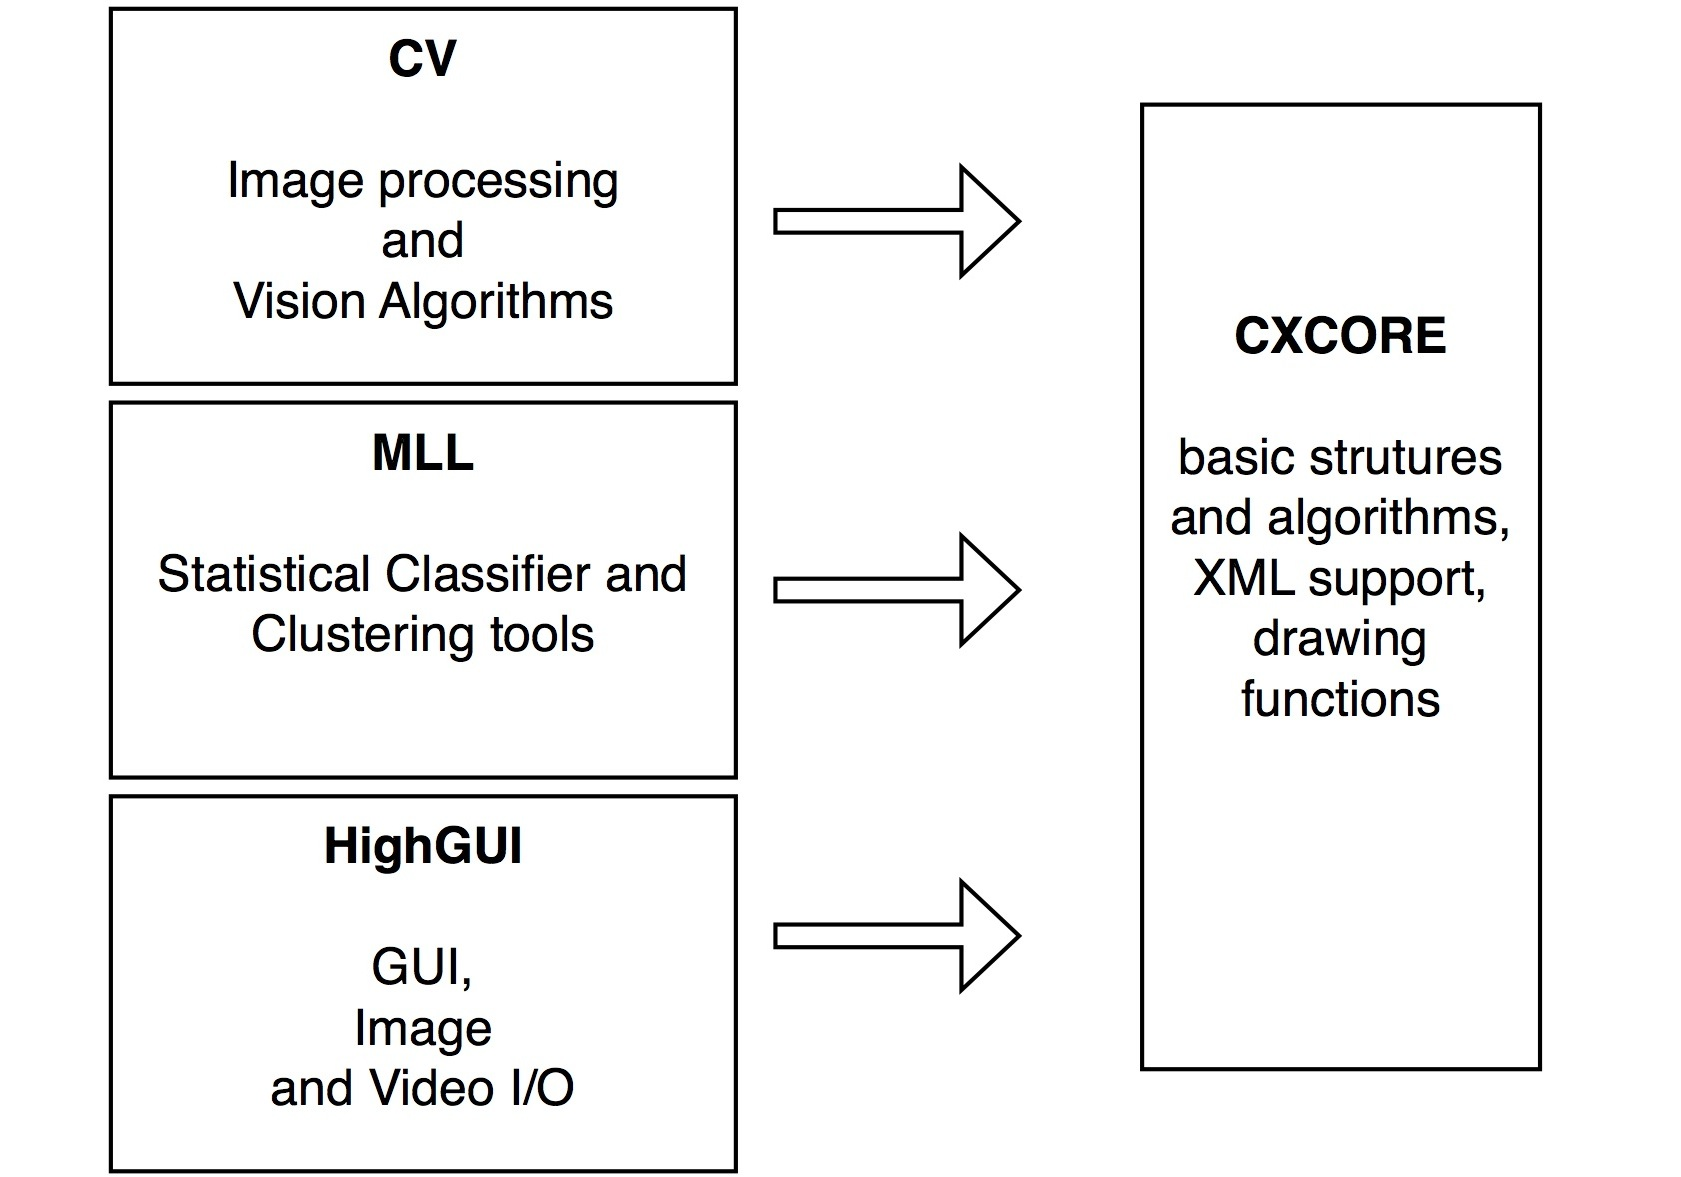
\includegraphics[width=110mm]{img/opencv_structure.jpg}}
    \caption{The basic structure of OpenCV library.}
\end{figure}
CXCore provides the core functionality including \todo{ten seznam prosim predelejme tak, aby byl spravne typograficky: mala pismenka a carky na konci radku krome posledniho zakonceneho teckou}:
\begin{itemize}
  \item Basic Structures
  \item Operations on Arrays
  \item Dynamic Structures
  \item Drawing Functions
  \item XML/YAML Persistence
  \item Clustering and Search in Multi-Dimensional Spaces
  \item Utility and System Functions and Macros.
\end{itemize}

In this part of OpenCV library we can find the basic structures that are needed for image processing.
They are represented as structures in the class Basic Structures. For example \stype{CvPoint} defines a point, \stype{CvSize} is a set of two numbers representing size of rectangle, 
\stype{CvScalar} is a container of double values, \stype{IplImage} is a structure inherited from the Intel Image Processing Library designed for loading images, 
or \stype{CvMat} is a data structure for storing a matrix.

As we can presume, the basic methods to work with these structures are implemented.
We can find there functions for mathematical operations on matrices such as multiplication (\stype{void cvMul()}), transposition (\stype{void cvTranspose()}), or
others like dividing multi-channel array into several single-channel arrays (\stype{void cvSplit()}).

Available are also drawing functions working with matrices or images including \stype{void cvCircle()} which as arguments takes an image, centre point of the circle,
and a colour and draws a circle in the image. Similarly \stype{void cvEllipse()} or \stype{void cvDrawContours()}.


The section with functions for image processing and computer vision provides these functionalities:
\begin{itemize}

  \item Image Filtering
  \item Geometric Image Transformations
  \item Miscellaneous Image Transformations
  \item Histograms
  \item Feature Detection
  \item Motion Analysis and Object Tracking
  \item Structural Analysis and Shape Descriptors
  \item Planar Subdivisions
  \item Object Detection
  \item Camera Calibration and 3D Reconstruction

\end{itemize}


\section{OpenCV4Android}
OpenCV library was written in C and this makes it portable to almost any commercial system.
Since the version 2.0, OpenCV includes also the new interface written in C++. \todo{predchozi vetu nevim proc rikame v sekci o androidu}
Later also wrappers for languages such as Java or Python have been developed. 
Since 2010 OpenCV was also ported to the Android environment, it allows to use the full power of the library in the development of mobile applications.
\todo{vubec cely tenhle odstavecek se hodi spis na zacatek kapitolky} 

In comparison with desktop version it also includes the \stype{opencv.android} package containing all the additional functions for the Android platform.
This package provides mainly an environment for work with camera by offering classes such as  \stype{NativeCameraView.java} or  \stype{CameraBridgeViewBase.java}.

